\section{Background}
By 2022, all\footnote{80\% by 2020} electrical meters in EU member countries will have been replaced by \textit{smart meters} \cite{smart_meter_survey} \cite{directive_2009_72_EC}.
An expansion of the power-line grid, as it is extended to connect more EU member countries, along with the addition of smart meters, enabling home owners to supply themselves and others, will form a smart grid.

\subsection{Smart Grid and Smart Meters}
The outline of a smart grid can be seen in \cref{fig:background:smartgrid}.
In the figure can be seen three main actors: power suppliers (Windmills, solar panels, power plants, external supplier), net supplier (Datahub, smart meters), and end consumers (Smart home and buildings).

The smart grid serves several purposes:
\begin{itemize}
	\item Adjusting prices based on supply and demand.
	\item Adjust prices based on type of energy available, as renewable energy is less dependable.
	\item Easily change energy supplier, in order to increase market competitiveness.
	\item Connect power-lines across Europe, greater enabling the three points above.
	\item Allowing users to monitor their own energy usage.
	\item Allowing users to adjust their energy consumption based on available energy/prices.
	\item Allowing users to be suppliers to the smart grid.
	\item Allowing users to use smart appliances, connected to the smart meter, allowing for home automation and optimized energy usage.
\end{itemize}

\begin{figure}
	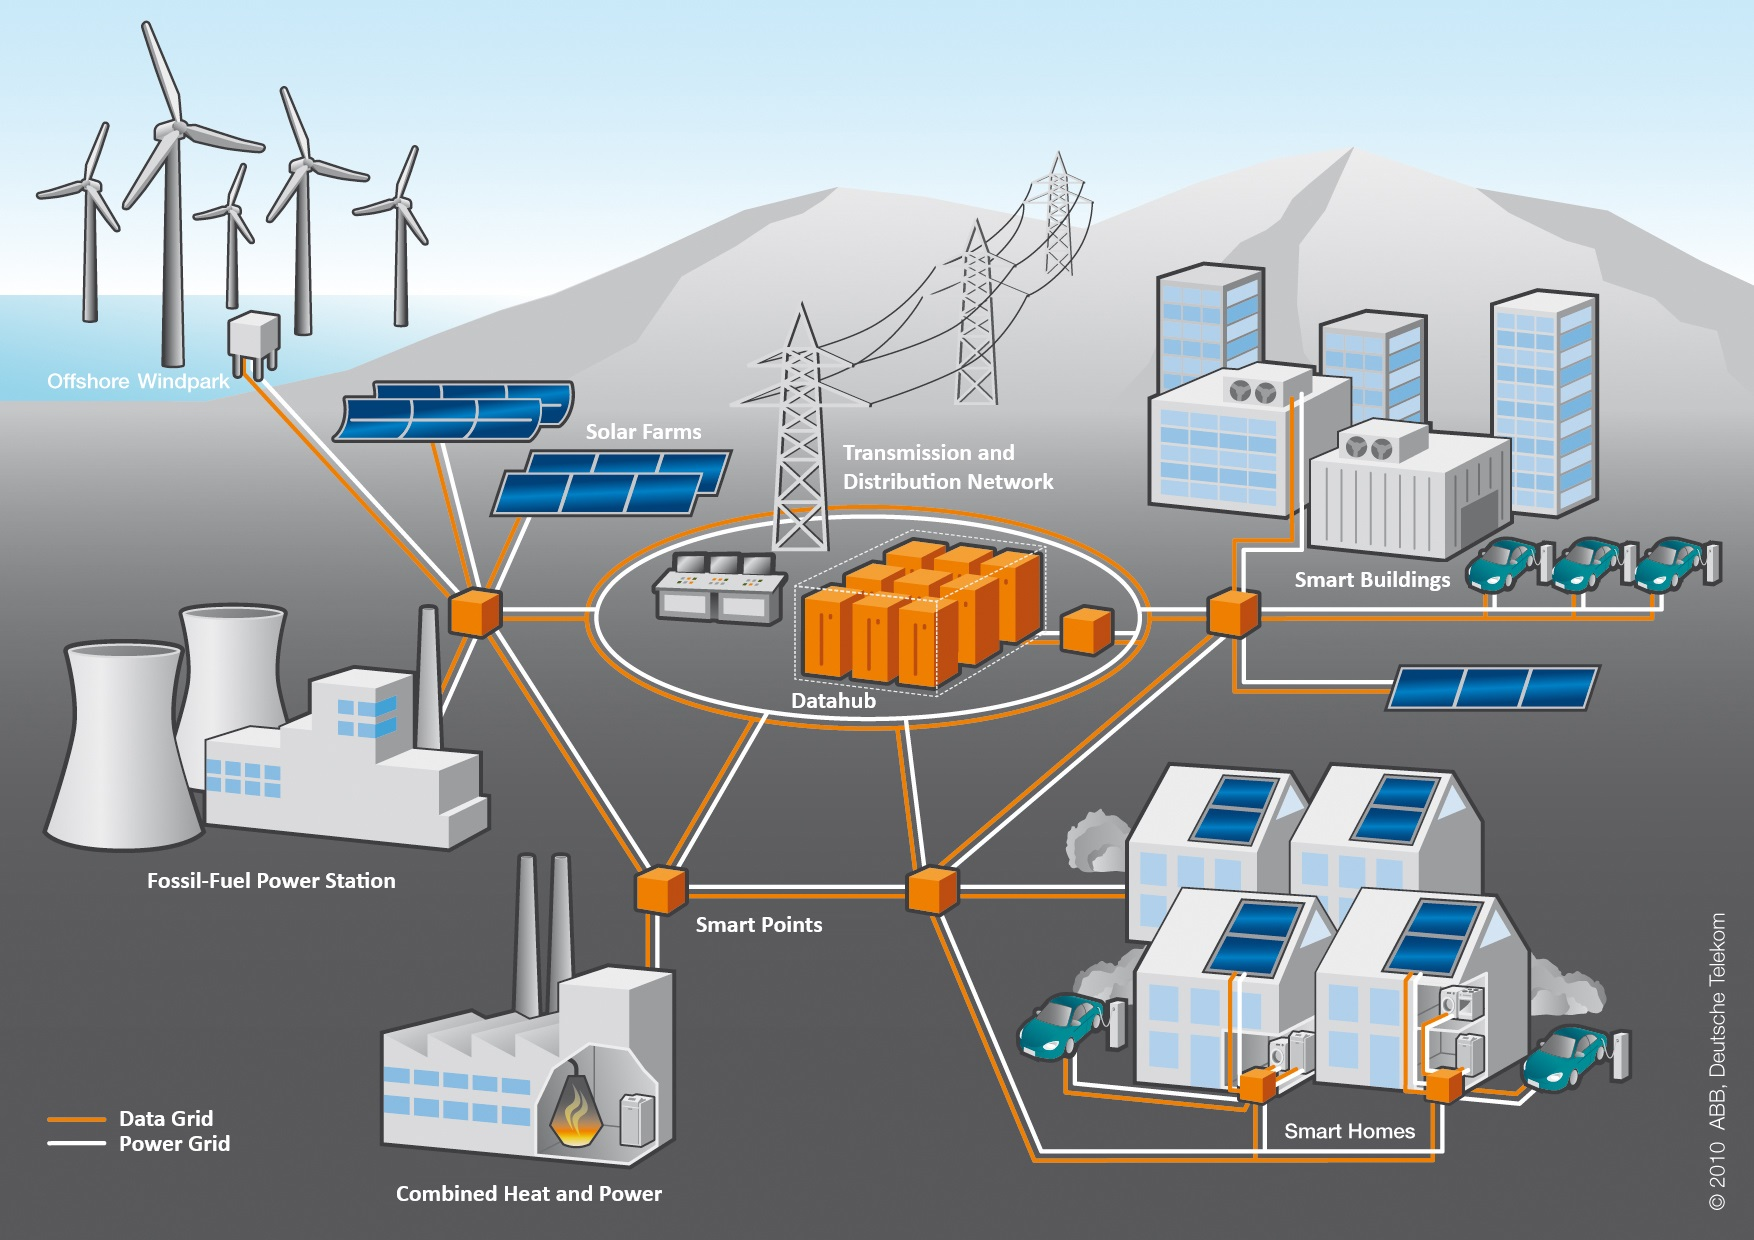
\includegraphics[width=\textwidth]{figures/SmartGrid_Ueberblick_ohneLegende.jpg}
	\caption{\url{http://powertown.no/wp-content/uploads/2011/11/SmartGrid_Ueberblick_ohneLegende.jpg} \url{https://www.telekom.com/medien/bild-ton-und-infografiken/infografiken/155030}}
	\label{fig:background:smartgrid}
\end{figure}

\subsection{Problems}

\paragraph{Different architectures}

\paragraph{Privacy}

\paragraph{Conflict of interest}

\paragraph{Vulnerabilities}
